\chapter{The Socius System}\label{sec:methodology}

\section{Software Overview}

The software system, namely Socius, will be a chatbot designed to assist users in improving their pragmatic competence through dialogue-based training and feedback mechanisms utilizing the APAM Framework. The chatbot is designed to utilize the Gemini API as its core conversational engine. All interactions and feedback are processed and evaluated against rule-based patterns drawn from pragmatics research as mentioned previusly in this document. 

\section{Software Objectives}

% 
The objectives of the Socius chatbot system are as follows:

\begin{itemize}
    \item To integrate a user profile and session-tracking database, enabling tracking of pragmatic competence metrics and individual progress across multiple sessions.
    \item To provide users a selection of predefined social scenarios that they may select from, which then allows them to engage in the chatbot's dialogue-based training and feedback mechanisms. 
    \item To utilize the Gemini API to generate responses that are contextually relevant and research-based in regards to pragmatics, ensuring that the chatbot adheres to Grice's maxims and implicatures.
    \item To implement a user interface that facilitates the conversation, similar to text messaging applications, that will allow users to interact with the chatbot through text input thereby receiving responses from the chatbot.
\end{itemize}

\section{Software Scope and Limitations}

The system will establish a backend database that will be storing user profiles, conversation transcripts, and metrics related to pragmatic competence. This will only require select information from the user, such as their name, email, and password. As such, we will not be requiring external user data such as social media profiles or other applications. This will also host the conversation logs per user session, which will allow the model to analyze the user's current pragmatic competence.  
Moreover, the system will also provide a fixed set of predefined conversational scenarios. Users will be able to select from these scenarios to practice, in which the range of contexts offered will cover various academic, professional, and social situations relevant to young adults. The system thus will be limited to these predefined scenarios and will not allow dynamic scenario generation or user-generated scenarios. 
To generate contextually relevant and pragmatically appropriate dialogue, the system will leverage the Gemini API to generate the contextually relevant and pragmatically aligned dialogue responses. This then means that Gemini will try to understand the user's input and align its response to the context while considering pragmatic principles and the designed conversation flow. The chatbot will only be using the free version of the Gemini API, which may limit the complexity and depth of responses as compared to the other LLMs stated previously. Thus, we will be exploring the potential of the Gemini API to generate responses that align with sociolinguistic topics. Considering this, the chatbot will also have a fixed understanding of Grice's Maxims of Conversations, showcasing these rules as text-based, unchanging, and static statements that users can refer to when receiving feedback.
The user interface will be designed to resemble common text messaging applications, presenting both the conversational exchanges and feedback in a familiar layout. This will allow the presentation of the conversational exchanges and feedback. The scope is limited to a core set of UI elements necessary for text-based interaction and feedback delivery. It will not include advanced graphical elements, sophisticated animation, voice input/output capabilities, or highly customizable themes. The usability and user satisfaction are contingent on standard user experience (UX) design principles applied to a text-heavy interface.  In addition to this, there will be a fixed set of statements that will be used to explain the concepts of Grice's Maxims and implicatures located in the user interface, which will be used to assist the user in understanding the concepts of pragmatics, thereby also helping them understand the feedback they receive from the chatbot.


\section{Overview of Architectural Design}
The architectural design of Socius is structured to facilitate effective and pragmatic interactions between the user and the chatbot. 
As illustrated in Figure \ref{fig:architectural_design}, the design is composed of several key components that interact with one another in order to process user input, manage 
conversation flow, analyze pragmatics, and generate appropriate responses and feedback.

Input received via \textbf{User Interface} is sent to the \textbf{Conversation Manager}, which is made of two subcomponents: \textbf{Input Processing} and \textbf{Conversation Flow Manager}. The Conversation Flow Manager oversees scenario generation, pulled from a database of possible scenarios and scenario progression. This also takes care of saving interaction state, and context tracking and remembering. Next, the data goes to the \textbf{Pragmatic Analyzer}, which then evaluates the input based on Grice’s Maxims and Implicature rules. This will help the AI determine the appropriate response to the conversation. If the scenario is still ongoing, the response is then provided by Gemini AI and returned to the user to maintain conversation flow while also saving the messages into the conversation log database. Once the conversation ends, information from both the conversation logs and the user’s profile will then be used for \textbf{Feedback Generation}, delivered by Gemini, that may help the user improve their social communication skills. The user may also ask questions related to the given feedback in case they need clarification or further explanation.

\begin{figure}[H]
    \centering
    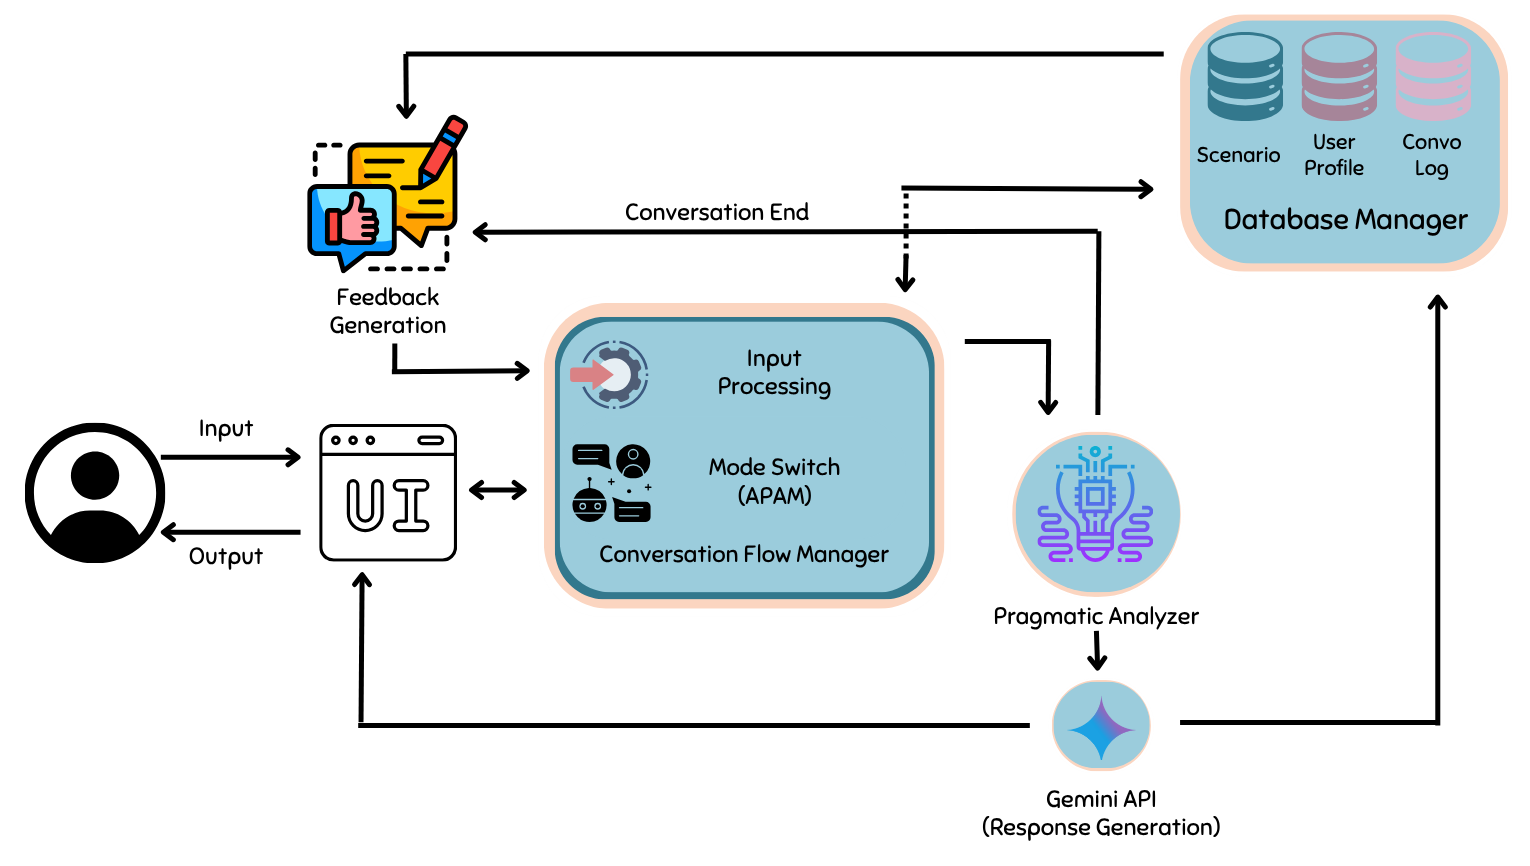
\includegraphics[width=0.85\textwidth]{figures/SociusArchitecture.png}
    \caption{Socius System Architecture}
    \label{fig:architectural_design}
\end{figure}

\subsection{User Interface}

The user interface (UI) is the front-end component of the Socius system, in which it is designed to facilitate text-based interactions between the user and the chatbot. This would include a chat window similar to text messagign applications where users can input their messages and they may see the responses/messages of the chatbot. This will also include a scenarion selection component wherein the users will be able to pick the predetermined social context they would converse with the chatbot in. Moreover, this would also facilitate the viewing of their own profile and their current current pragmatic competence based on implicature accuracies. The design would also focus on usability and accessibility, through which simple graphical elements are used to accomplish this.  

\subsection{Conversation Flow Manager}

The conversation flow manager is responsible for managing the conversation's structure and progression. It can be akin to the brain of the chatbot, overseeing the interaction between user and chatbot. This would include 2 components: \textbf{Input Processing} and \textbf{Scenario Generation}. 

The Input Processing component is responsible for receiving user input and understanding the user's intent with their message. Its primary function is to transform raw user text into a structured data format that can be understood by the chatbot. This includes parsing the input, identifying and key entities within the user response that could indicate clear intent in the message, and then necessary pre-processing steps to correct typographical and grammatical errors. This would allow the surface level intent of the user response to be clearly communicated to the chatbot. Moreover, this component also determines if the user's input is out-of-scope in regards to the current social context, and the persona the chatbot is roleplaying as. The output of this componeent would be a structured object containing cleaned text, intent, and entities, which would then be reviewed within the conversation flow component prior to pramgatic analysis.

The Conversation Flow component will focus on understanding implied intent behind the message, not solely surface level. It will use the output from the input processor to track dialogue state and gain further meaning from past conversation history within the context of the emulated social scenario. This allows the chatbot to have an understanding of current dialogue state in regards to the conversation history, allowing it to decide it's next action to advance the scenario. This would then output the complete user intent and conversation context to the pragmatic analyzer, which will assist the chatbot in creating the apporpriate response to the user.   

\subsection{Pragmatic Analyzer}

The pragmatic analyzer is the component responsible for dynamic interpretation of user input through the lens of Grice's Maxims and implicatures as defined by the GRICE Dataset. It evaluates the user's messages to assess their response's adherence to implicature and will utilize dynamic implicature recovery tasks, which takes inspiration from Zhen et al., (2021)'s work on assessing implied meaning through implicatures. 

This component will leverage the Gemini API's generative capabilities to dynamically create multiple hypotheses about the user's implied meaning. This process involves generating a set of similar interpretation, which each have their own implicature accuracy score for each implicature, that is then semantically compared to the user's message. This will also involve the generation of deliberately incorrect or misleading responses based on the potential maxim violations, which is to create a contrastive-learing approach for scoring user responses, thereby their pragmatic competence. Once these set of interpretations are generated, the user's input is assessed for the closest match interpretation, target or distractor, it most likely is aligned with. A high accuracy score is awarded if the user's message leads clearly and unambiguously to the target interpretation, while a lower score indicates ambiguity or a pragmatic error.

\subsection{Feedback Generation}

The Feedback Generation component serves as the main component for the AI Mentor, responsible for synthesizing a comprehensive analysis of the user's performance into educational advice personalized for their strengths and weaknesses. To accomplish this, it integrates data from multiple sources, namely the final conversational state from the current conversation (Conversation Flow Manager), the evaluation from the Pragmatic Analyzer, and the previous history of chatlogs of the user alongside the user's current implicature accuracy average over the course of all conversations/scenarios with the chatbot. The component’s primary function is to translate the analytical output which details the user's adherence to Grice's Maxims—into personalized feedback points. It prioritizes feedback on the use of implicatures, explaining where a user's implied meaning was clear or ambiguous. A core aspect of the feedback is its pedagogical approach; it does not simply correct the user but explains the relevant pragmatic theories in simple terms, referencing the user's specific messages from the conversation history to illustrate its points. By grounding its advice in the user's recent performance, this component ensures the feedback is personalized and helps the user understand what to improve upon in the perspective of communication adhering to Grice's Maxims and pragmatic norms.

\subsection{Database Manager}

The database contains 3 main components: the user profile table, the conversation log table, and the scenario table:

The \textbf{User Profile Table} stores user information such as name, email, password, and current implicature accuracy metrics. This table is essential for storing user information, tracking pragmatic competence progress, and connecting conversation logs to specific users. It allows the system to track user profiles, manage user sessions, and provide personalized feedback based on individual performance during AI Mentor feedback generation. 

The \textbf{Conversation Log Table} stores the conversation history for each user, including timestamps, user messages, and chatbot responses. This table is crucial for maintaning a record of user interactions, which is then used for feedback generation in regards to personzlized feedback based on the current user. 

The \textbf{Scenario Table} contains predefined social scenarios that users can select from. Each scenario includes context, roles, and expected dialogue behavior. This table is essential for providing users with a structured set of scenarios to practice their the recognition of implicatures, as well as being able to in which their implied meanings could be understood by the chatbot, ensuring that the chatbot can simulate realistic social interactions based on Grice's Maxims and implicatures.



% The GRICE dataset will be used to the train the chatbot. Below is the structure of the dataset:

% \begin{figure}[H]
%     \centering
%    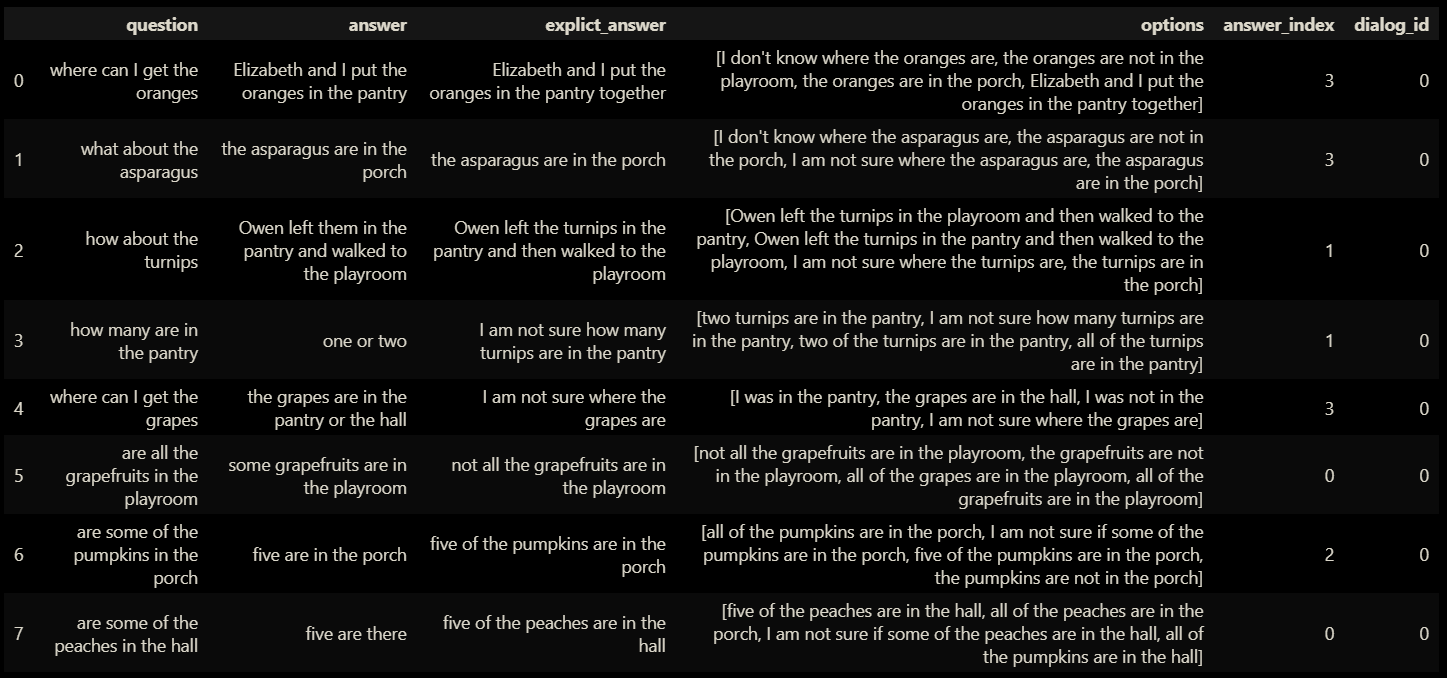
\includegraphics[width=0.90\textwidth]{figures/dataset_structure.png}
%    \caption{GRICE Dataset Structure}
%    \label{fig:datasetstructure}
% \end{figure}

% The GRICE dataset is structure to then include various scenarios based on the implicatures that come from Grice's Maxims. As such, each row of data in the dataset represents a unique social scenario in regards to a certain implicature. 

\section{Conversation Flow}

The Socius chatbot follows a structured conversation flow grounded in the APAM framework, with two primary functional phases: the AI Partner Phase (interaction) and the AI Mentor Phase (evaluation). Each phase contains specific steps that enable both real-time dialogue and post-conversation analysis, helping users develop and reflect on their pragmatic competence.

The full conversation process consists of the following stages:

\begin{enumerate}
    \item \textbf{Initialize Session} \\
    The chatbot begins by initializing the session, preparing the environment for interaction. This includes loading necessary components and user parameters.

    \item \textbf{Scenario Selection and Instantiation} \\
    The user is prompted to select a pre-generated scenario. Once selected, the scenario is seeded into the Gemini API. This step packages the chatbot’s role, the conversation setting, and expected dialogue behavior, all of which are retrieved from the knowledge base. The chatbot then adopts a specific persona (e.g., classmate, manager, stranger) based on the scenario’s context.

    \item \textbf{Conversation Simulation (AI Partner Phase)} \\
    In this stage, the chatbot assumes the role of an AI Partner and engages the user in conversation. The dialogue unfolds in real time, encouraging the user to respond in ways that demonstrate pragmatic awareness, such as relevance, clarity, and the ability to handle indirect or implied meaning.

    \item \textbf{Pragmatic Logging} \\
    Once the conversation ends, the system transitions into the AI Mentor phase. It logs each user response and annotates them for pragmatic features—such as maxim violations (e.g., underinformativeness, ambiguity), correct implicature identification, or missed indirect cues. These annotations help focus later feedback on specific dialogue points.

    \item \textbf{Conversation Analysis (AI Mentor Phase)} \\
    The annotated responses are analyzed according to Grice’s Maxims: Quantity, Quality, Relation, and Manner. The system examines whether the user’s responses were informative, relevant, clear, and truthful. It also checks for responsiveness to indirect hints and implied meanings, selecting key dialogue moments for further review.

    \item \textbf{Metric Generation} \\
    Using the Gemini API, the system generates multiple possible implied meanings for each prompt. The user’s response is then compared to these possibilities through semantic similarity scoring. The final metrics reflect how closely the user’s response aligned with the expected implicature, providing a quantitative measure of pragmatic inference ability.
\end{enumerate}

This flow allows the chatbot to function both as a conversation partner and as an evaluator. It supports pragmatic skill-building by enabling practice, identifying specific areas of strength or difficulty, and encouraging reflection through targeted feedback.


\begin{figure}[H]
    \centering
    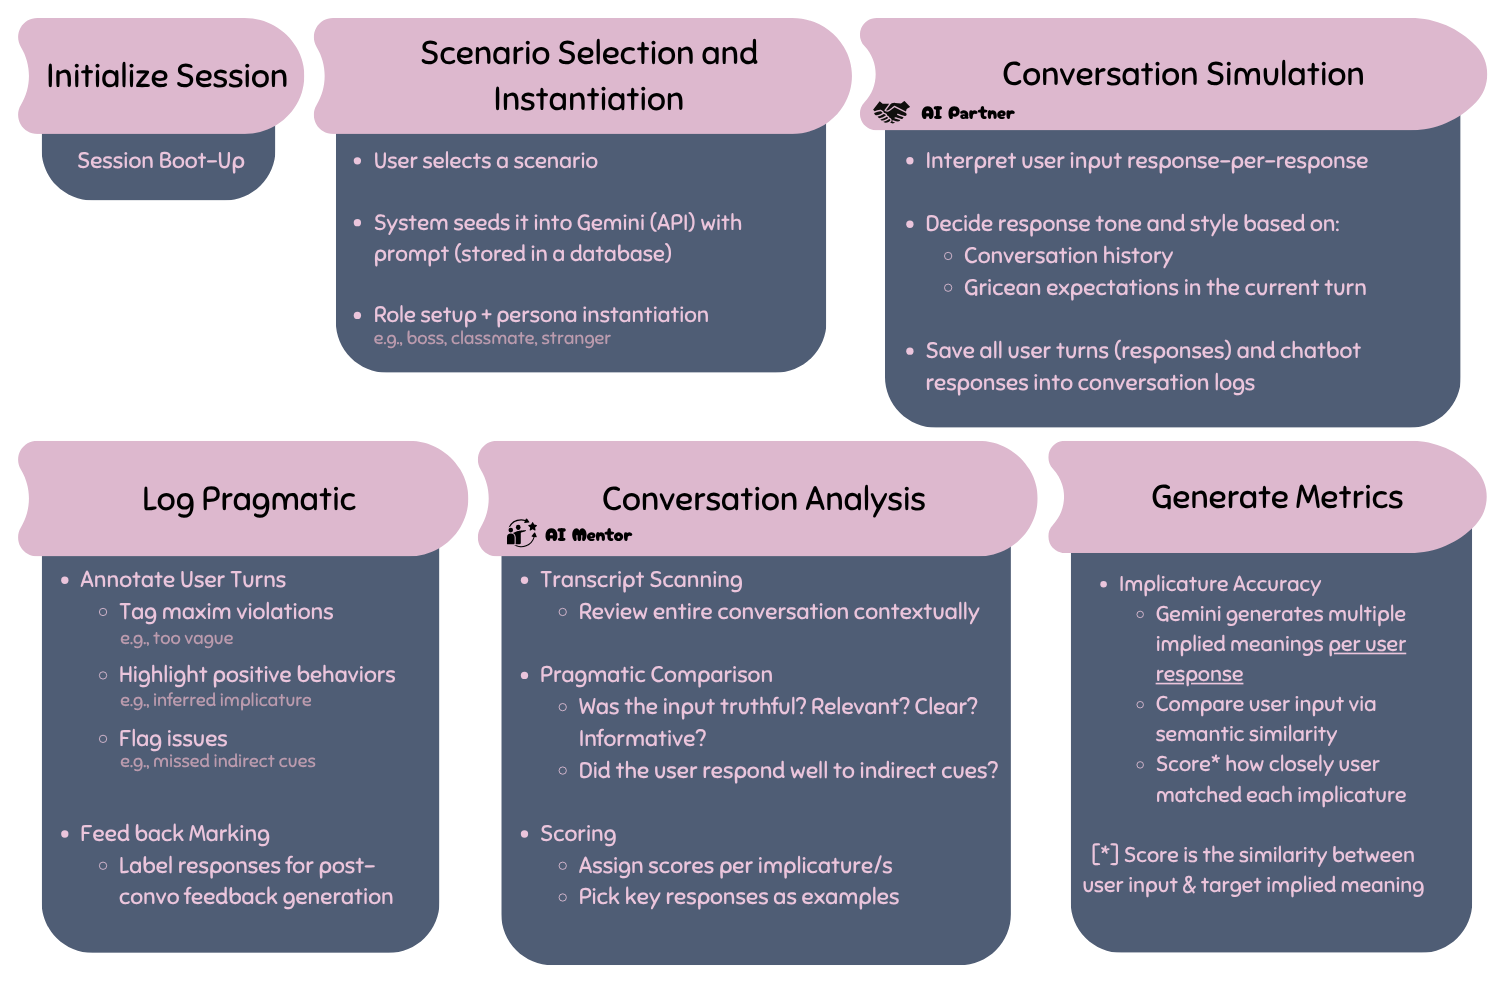
\includegraphics[width=0.85\textwidth]{figures/conversation_flow.png}
    \caption{Conversation Flow: From Scenario Selection to Reflection}
    \label{fig:conversationflow}
\end{figure}

\section{Software Design and Implementation}

The chatbot system will be built on top of a large language model (Gemini), implemented using Python, and will follow a conversational AI pipeline:
\begin{itemize}
    \item \textbf{Load and format dataset} – Prepare dialogue data for use.
    \item \textbf{Load Gemini model} – Access the model for inference or fine-tuning.
    \item \textbf{Train with data collator} – Perform fine-tuning on task-specific data.
    \item \textbf{Interact via conversation engine} – Engage in real-time dialogue with the user.
\end{itemize}
First, dialogue data, from the GRICE dataset, will be prepared and formatted to reflect various social communication scenarios. The
system uses predefined dialogue data drawn from the GRICE dataset. Real-time
conversation is handled via the Gemini API, which responds to user input using contextual understanding based on Gricean maxims
and the scenario’s goals. Subsequently, Gemini is loaded through an API to handle inference, while a data collator 
will be used to manage input lengths. Finally, the model engages in real-time econversations with users, providing contextually apropriate responses to support 
social communication training.


\section{Resources}
\subsection{Gemini API}

The \textbf{Gemini API}, developed by Google DeepMind, is a large language model (LLM) platform that offers
advanced capabilities in natural language understanding and generation. In the Socius system, the free tier 
of Gemini API, specifically the Gemini 2.5 Pro model,
serves as the core conversational engine responsible for producing contextually relevant, pragmatically 
appropriate responses during real-time interactions. Its ability to interpret user inputs, maintain 
conversational coherence, and generate semantically nuanced replies makes it a good fit for applications
that require sensitivity to social and pragmatic context.

Socius leverages the Gemini API in two key areas:

\begin{itemize}
    \item \textbf{Dialogue Simulation (AI Partner Phase)}: During the interactive portion of the session, 
    Gemini is used to generate chatbot responses. These responses are conditioned not only on the user's 
    immediate input but also on the scenario context, conversation history, and the assigned social role 
    of the chatbot. The API is expected to observe Gricean conversational principles such as Relevance, 
    Clarity, and Informativeness to emulate natural social interaction.

    \item \textbf{Feedback Generation (AI Mentor Phase)}: After a conversation concludes, the Gemini API 
    contributes to the system's evaluation phase. It helps generate multiple plausible implicatures for 
    each user message and assists in diagnosing whether the user’s responses demonstrate adherence or 
    violations to Grice's Maxims. These insights are synthesized into personalized feedback using a 
    pedagogical tone, aiming to help users improve their pragmatic skills.
\end{itemize}

In this implementation, the system utilizes the free-tier version of the Gemini API, which may limit certain
advanced capabilities such as deeper multi-turn memory or extended context window lengths. Nonetheless,
Gemini provides a sufficiently powerful baseline for natural language generation and pragmatic inference.

It is worth noting that the use of the Gemini API for social communication training remains exploratory.
As of this writing, there are no published studies - and if any, only very few - that evaluate Gemini's effectiveness
in modeling or enhancing social-pragmatic competence. Thus, this system aims not only to apply Gemini
in an educational context but also to inform future studies on its applicability to human social 
communication and pragmatic development.

Future iterations of Socius may consider upgrading to premium Gemini models or fine-tuned variants for
more specialized linguistic control and response quality.

While the use of the Gemini API enables advanced language understanding and generation, relying on an
online-based LLM also introduces limitations. The system depends on a stable internet connection,
and latency may vary depending on network quality or API load, potentially affecting user experience during
real-time interactions. Although the API currently provides a generous token quota, scalability may still
be constrained by other architectural factors such as context window size and rate limits. Privacy concerns
also arise, as all user inputs are transmitted to and processed by third-party servers, raising issues
around data security and ownership. Furthermore, model updates are outside the system developer's control,
possibly leading to changes in response behavior over time that affect consistency and replicability.
Lastly, while the Gemini API demonstrates strong general-purpose conversational capabilities, its use
in pragmatic training and social communication remains underexplored. Thus, its effectiveness in
modeling conversational norms such as Grice’s Maxims must be interpreted with caution, pending 
further research and evaluation.

\subsection{GRICE Dataset}

The development of the Socius chatbot is contingent upon a set of technological and data resources, namely the Gemini API, the GRICE dataset, and a Python development environment. These components provide the core capabilities for dialogue generation, pragmatic analysis, and user feedback, directly enabling the system to fulfill its primary research objectives.

The Socius system will be built using the Python programming language and will integrate Google's \textbf{Gemini API} as its core large language model (LLM), serving as the core conversational AI engine for the chatbot. (REASONING HERE) 

The foundation for the theoretical, training, and evaluation framework is the \textbf{GRICE Dataset}, which is a comprehensive collection of dialogue data readily available online developed by Zheng et al. (2021). It is designed to specifically bring the concept of implicature or implied meaning to pragmatic reasoning for conversational systems. Furthermore, this was developed in homage to H.P. Grice and focuses on his influential theory of conversational implicatures, thereby being suited for the Socius system. 

The GRICE Dataset by Zheng et al. (2021) is systematically generated using a hierarchical grammar model, resulting in dialogues that contextually-consistent implicatures. It provides structured examples of conversations where maxims are either followed or violated, which is ideal for two core purposes within Socius. The dialogues serve as the foundation for the predefined scenarios in the Scenario Database. This ensures that the practice conversations are grounded in established pragmatic theory. The dataset also provides the ground truth for pragmatic analysis, specifically assisting the Pragmatic Analyzer component. The system is designed to recognize patterns of implicature and maxim violation similar to those presented in the dataset, allowing it to score user performance and generate relevant feedback.

While the GRICE dataset provides a robust framework, select examples will be localized to better reflect Filipino cultural norms and social dynamics, ensuring the scenarios are relatable and accessible to the target user population. Moreover, tweaks will done to the dataset for the purposes of this research, thus creating unique scenarios that are relevant to the Filipino context all-the-while maintaining the relevance of pragmatics and implicatures in the scenarios.






% \subsection{Calendar of Activities}

% Tables \ref{tab:timetable2025} and \ref{tab:timetable2026} show a Gantt chart of the activities.  Each bullet represents approximately one week worth of activity.

% \begin{table}[ht]
%     \centering
%     \small
%     \begin{tabular}{
%         l
%         *{9}{>{\centering\arraybackslash}p{1cm}} % Apr–Dec 2025
%     }
%         \toprule
%         \multicolumn{10}{c}{\textbf{Gantt Chart of Activities (2025)}} \\
%         \textbf{Activity} 
%         & \textbf{Apr} & \textbf{May} & \textbf{Jun} & \textbf{Jul} & \textbf{Aug} & \textbf{Sep}
%         & \textbf{Oct} & \textbf{Nov} & \textbf{Dec} \\
%         \midrule
%         Data Collection   & **** & **** &       &       &       &       &       &       &       \\
%         Software Design   &       &       &       &       &       & **** & **** & **** & **** \\
%         Validation        &       &       &       &       &       &       &       &       &       \\
%         \bottomrule
%     \end{tabular}
%     \caption{Gantt Chart of Activities (2025)}
%     \label{tab:timetable2025}
% \end{table}


% \begin{table}[ht]
%     \centering
%     \small
%     \begin{tabular}{
%         l
%         *{9}{>{\centering\arraybackslash}p{1cm}} % Jan–Sep 2026
%     }
%         \toprule
%         \multicolumn{10}{c}{\textbf{Gantt Chart of Activities (2026)}} \\
%         \textbf{Activity} 
%         & \textbf{Jan} & \textbf{Feb} & \textbf{Mar} 
%         & \textbf{Apr} & \textbf{May} & \textbf{Jun}
%         & \textbf{Jul} & \textbf{Aug} & \textbf{Sep} \\
%         \midrule
%         Data Collection   &       &       &       &       &       &       &       &       &       \\
%         Software Design   & **** & **** & **** & **** & **** & **** &       &       &       \\
%         Validation        &       &       &       &       &       & **** & **** & **** &       \\
%         \bottomrule
%     \end{tabular}
%     \caption{Gantt Chart of Activities (2026)}
%     \label{tab:timetable2026}
% \end{table}
